\documentclass[11pt, a4paper, twoside]{article}

\usepackage{graphicx}
\usepackage{geometry} % Adjust left margin to 4cm and right margin to 1cm
\usepackage{url} % Required for \url{}
\usepackage{xcolor} % Required for specifying colors by name
\usepackage{subcaption}
\usepackage{hyperref}
\usepackage{float}
\usepackage[utf8]{inputenc} % Enable UTF-8 encoding
\usepackage{titlesec}
\usepackage{mfirstuc}
\usepackage{lipsum}
\usepackage{helvet}
\usepackage{changepage} % for the adjustwidth environment
\usepackage{fancyhdr}
\renewcommand{\familydefault}{\sfdefault}
\usepackage{caption}
\usepackage{multicol}


\begin{document}
\title{RC11 Workshops}
\author{Joris Putteneers}
\date{}
\maketitle
% first assignment

	\section*{houdini fundamentals}

This session coveres the houdini fundamentals. For the exercice, the
following is expected.

	\begin{itemize}
		\item 

Alter 2 of the example setups we covered during class.
This means, add / remove minimim 2 nodes to a setup. Changing the parameters is
not enough. Adding a Null sop or adding unconnected nodes does not count.

	 	\item 
describe in the most detail what exactly your setup is doing. some important
keywords and terminology are  \textit{ node, parameter,
procedural, datatype, attribute, class, geometry, point, primitive, vertex,..}. Obviously, the example below cannot be used.
 
	\end{itemize}	
	An example of such a description would be :

	% overview image
	\begin{figure}[h]
		\centering
		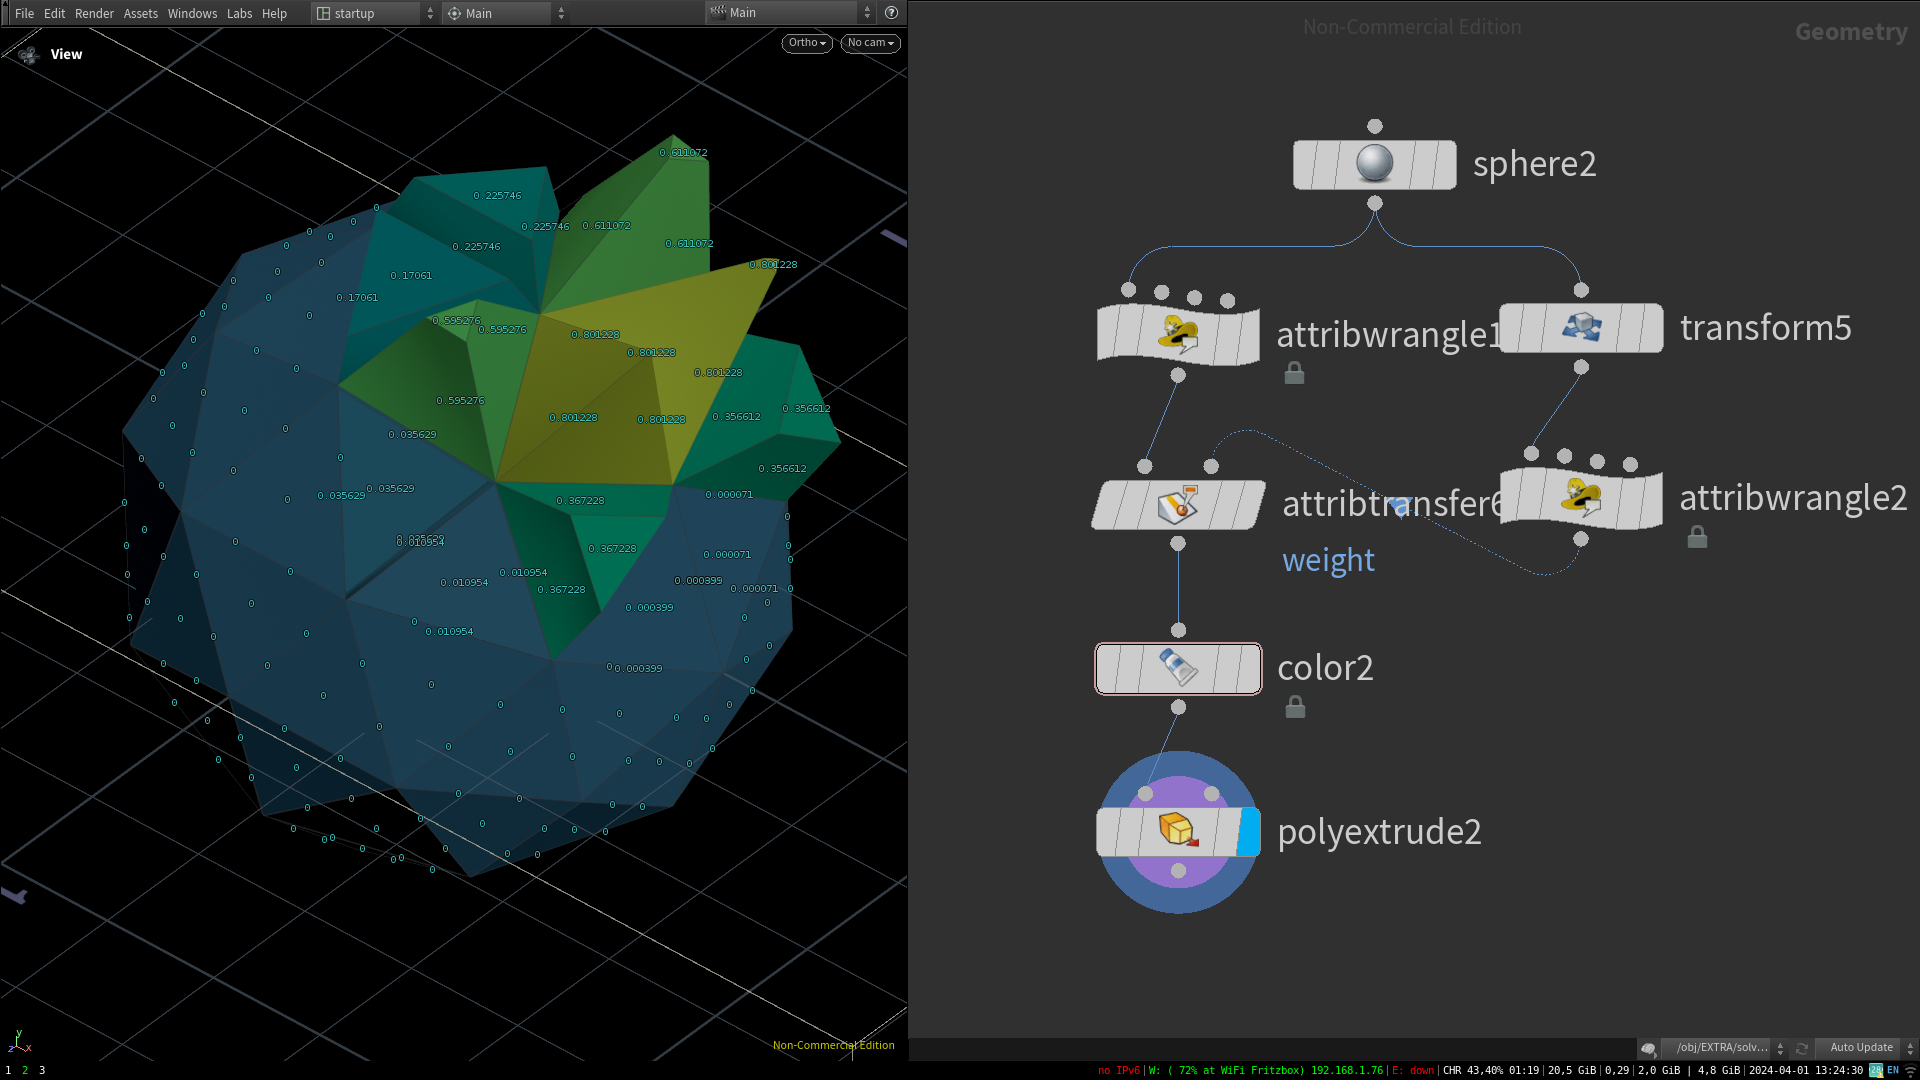
\includegraphics[width=\textwidth]{media/houdini_fundamentals_overview.png}
		\caption{houdini fundamentals: setup 1 overview}
		\label{fig:assignment1}
	\end{figure}

	%begin first image
	\begin{minipage}[H!]{0.4\textwidth}
		\textbf{1: sphere SOP} \newline 

A sphere is created. the sphere is
of primitive type: polygon. Once of the basic datatypes that contains: points,
primitives of type: polygon, and vertecis.  

	\end{minipage}
	\vspace{1pt}
	\begin{minipage}[H]{0.6\textwidth}
		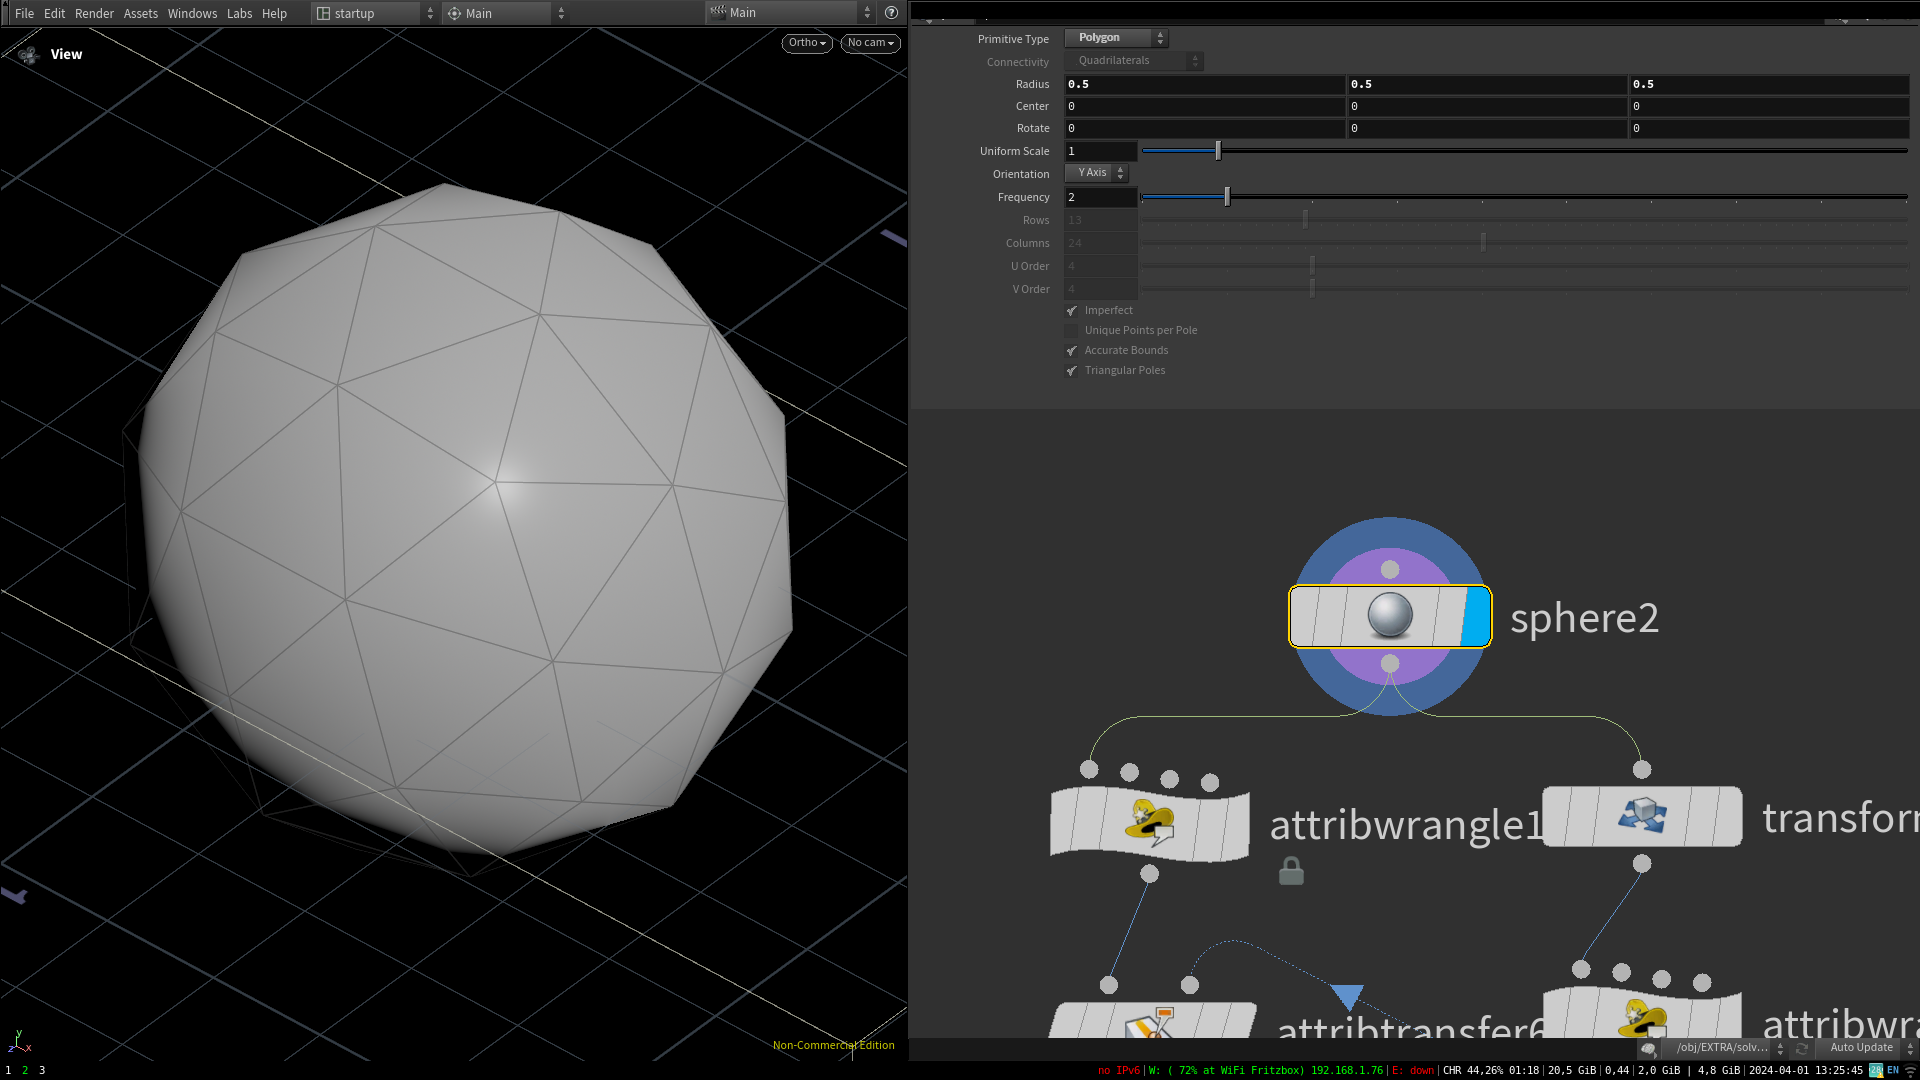
\includegraphics[width=1\textwidth]{media/houdini_fundamentals_1.png}
	\end{minipage}



	\begin{minipage}[H]{0.4\textwidth}
		\textbf{2: atribute wrangle SOP}\newline 

We create a attribute wrangle sop, where we make a "weight" attribute. the
attribute is of type float as described by the "f@" declaration. the attribute
is set to run over primitives, this is because later in the node setup, we will
use a polyextrude node where we will need a primitive attribute to drive the
extrusion value. The value is set to 0. (which will be interpreted as 0.0
because of the float declaration) because later, we can interpolate between 0
and 1. 
	
	 \end{minipage}
	\vspace{1pt}
	\begin{minipage}[H]{0.6\textwidth}
		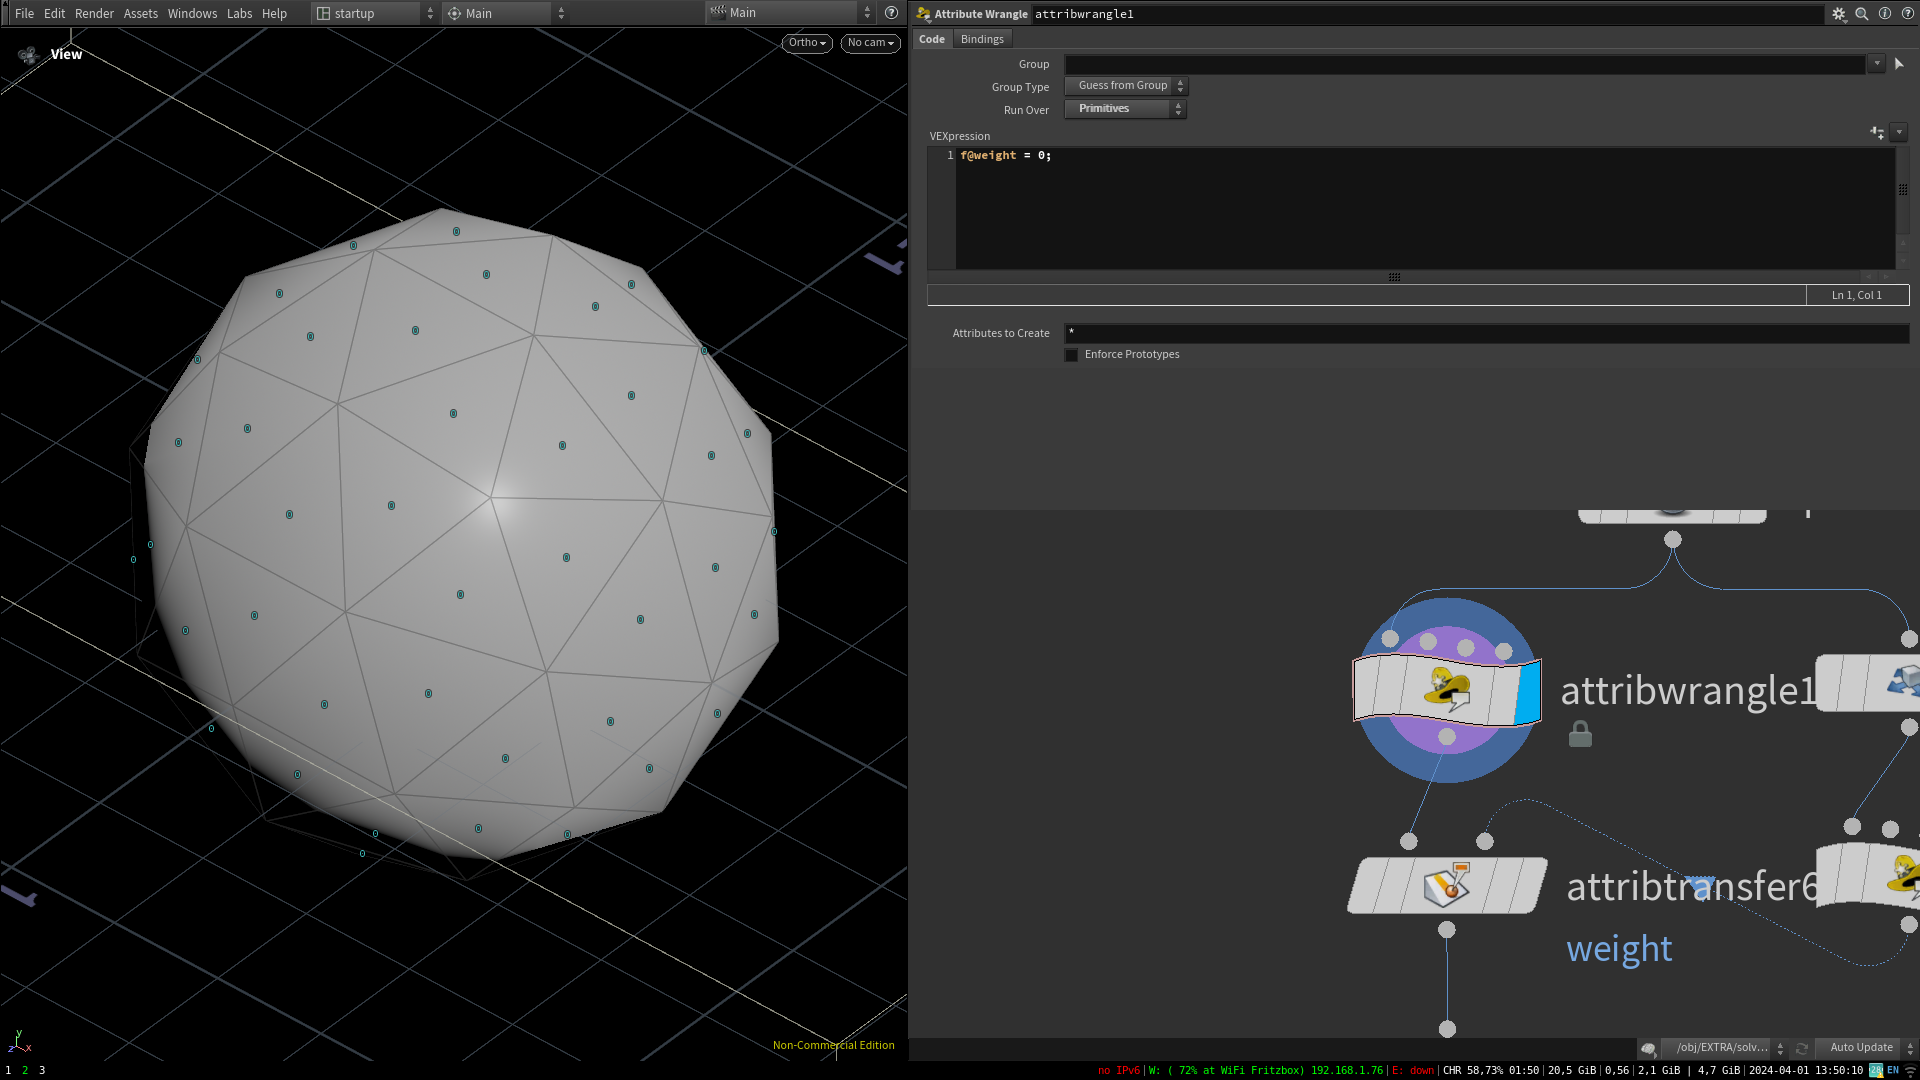
\includegraphics[width=1\textwidth]{media/houdini_fundamentals_2.png}
	\end{minipage}


	\vspace{10pt}

	\begin{minipage}[H]{0.4\textwidth}
		\textbf{3: transform SOP}\newline 

Then, i layed down a "transform" sop, This will be the attractor,it is just a
duplicate of the original sphere. the distance between this duplicate
(attractor) and the original sphere will dictate the final extrusion value. 
	
	\end{minipage}
	\vspace{1pt}
	\begin{minipage}[H]{0.6\textwidth}
		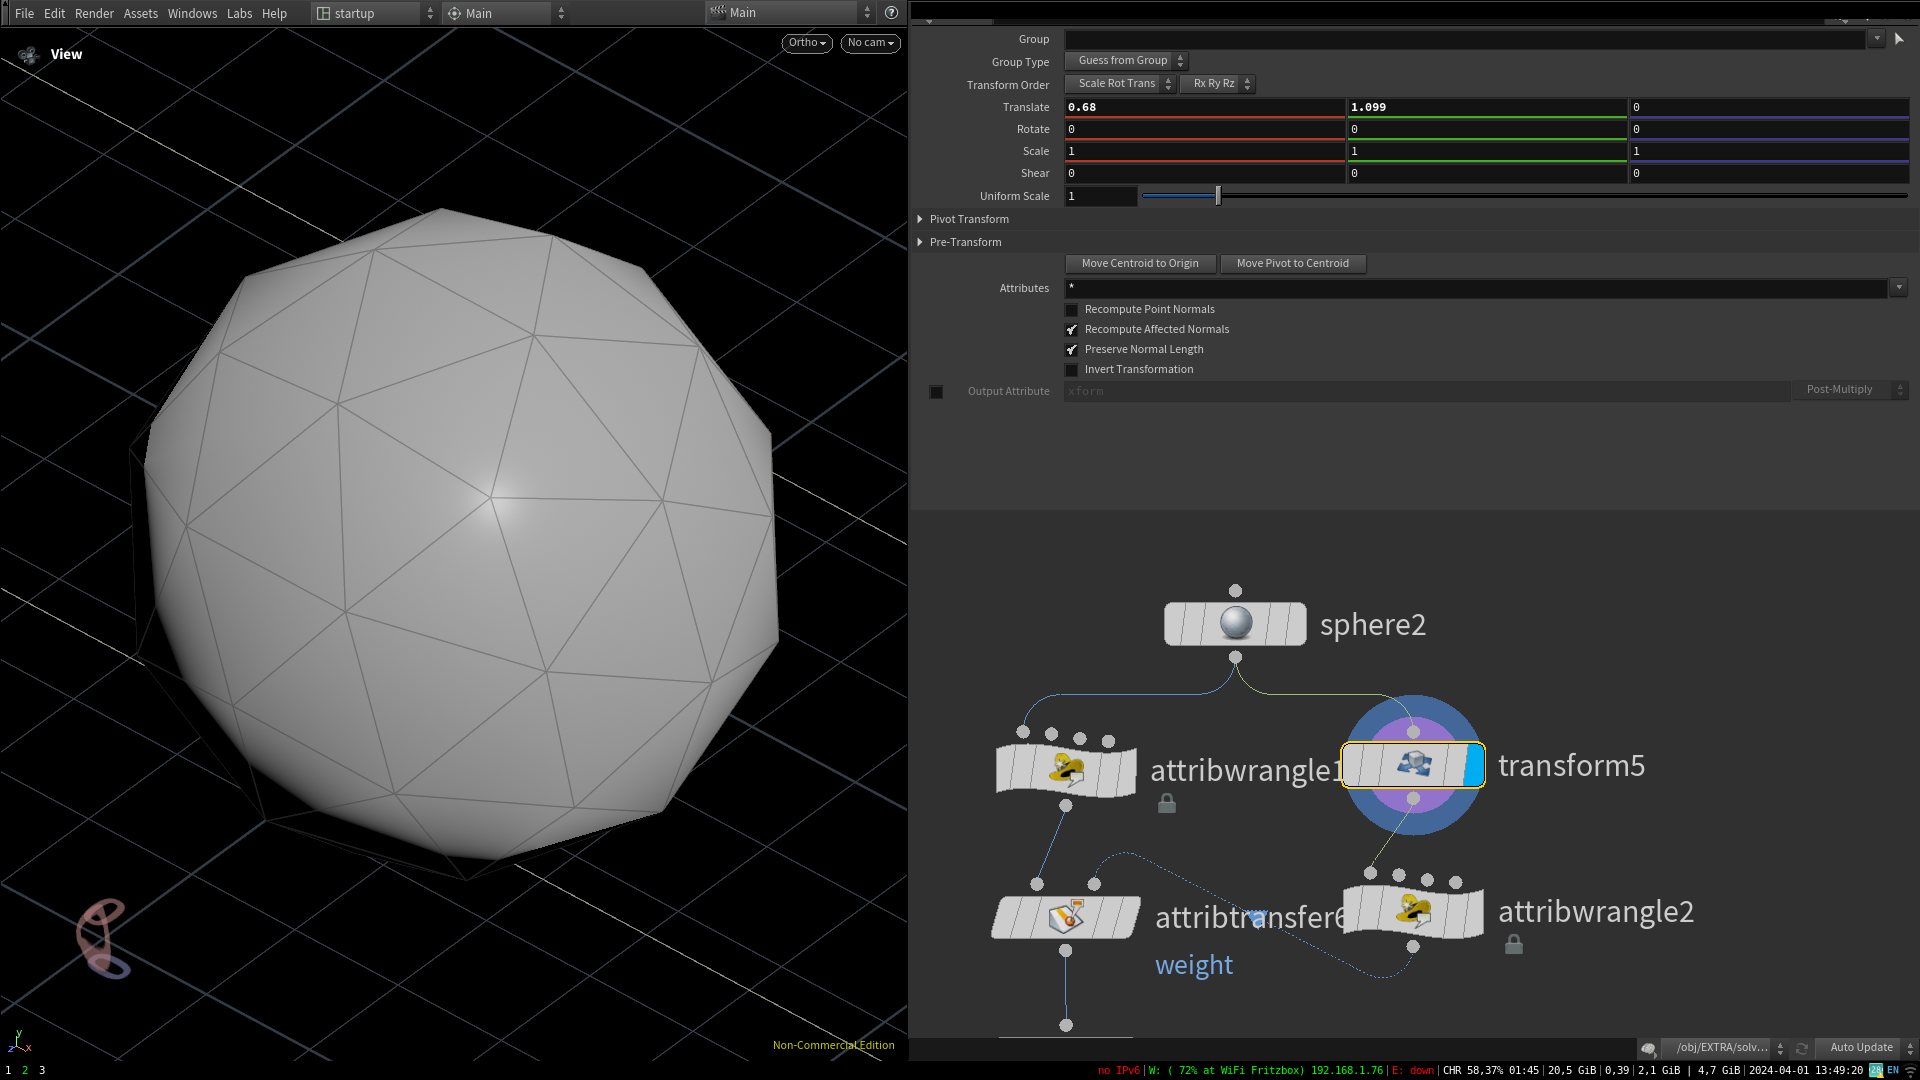
\includegraphics[width=1\textwidth]{media/houdini_fundamentals_3.png}
	\end{minipage}


	\begin{minipage}[H]{0.4\textwidth}
		\textbf{4: attribute transfer SOP}\newline 

the attribute transfer sop uses the "weight" primitive attribute to write out
the distance value between the original sphere and the attrcator. by setting the
originla 'weight' attributes as float, we can have value interpolations between
0 and 1. if we had set the weigt attributes to integers, we sould not
interpolate. the output values  would be binary (0 or 1). 
 
	\end{minipage}
	\vspace{1pt}
	\begin{minipage}[H]{0.6\textwidth}
		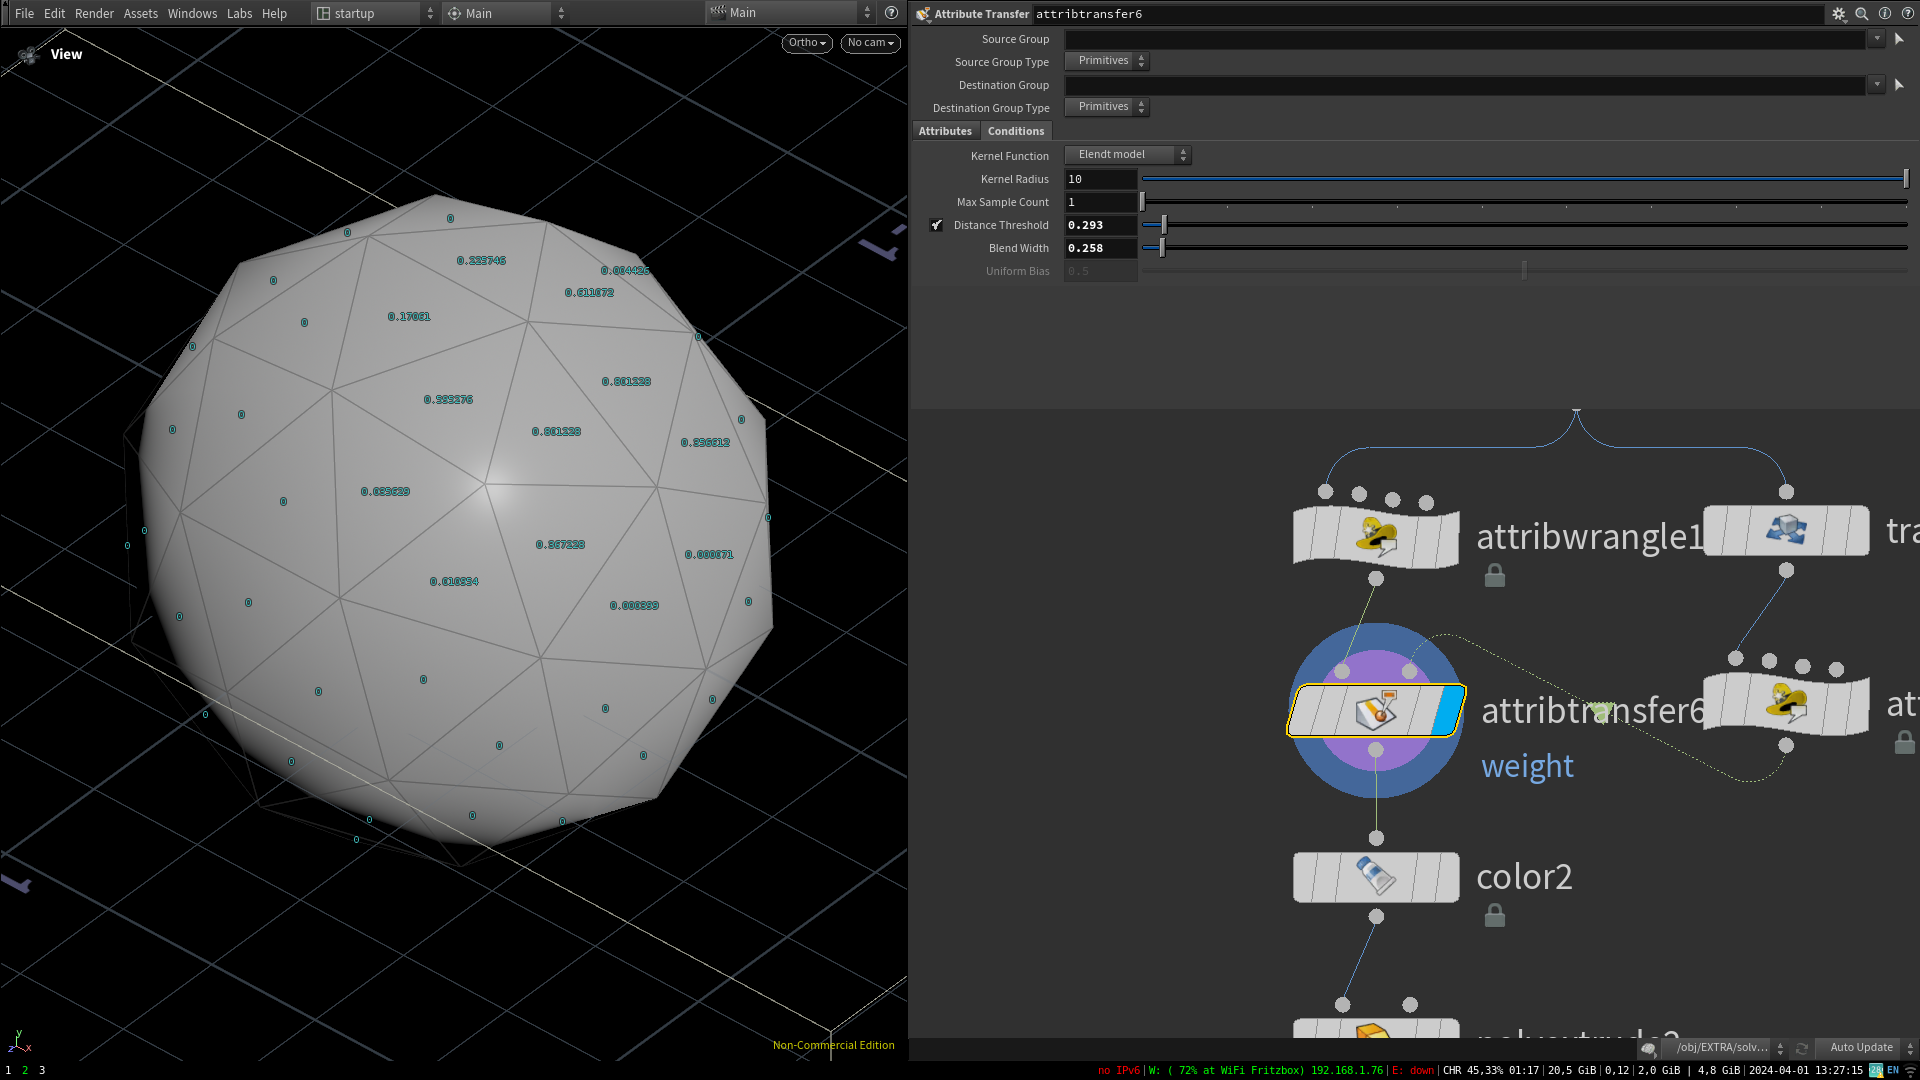
\includegraphics[width=1\textwidth]{media/houdini_fundamentals_4.png}
	\end{minipage}


	\begin{minipage}[H]{0.4\textwidth}
		\textbf{5: attribute wrangle SOP}\newline 
the same as the previous wrangle SOP, only with the opposite value.The reason
we interpolate between 0 and 1 is because it is easier to work with normalized
values that arbitrary values. 
	
	\end{minipage}
	\vspace{1pt}
	\begin{minipage}[H]{0.6\textwidth}
		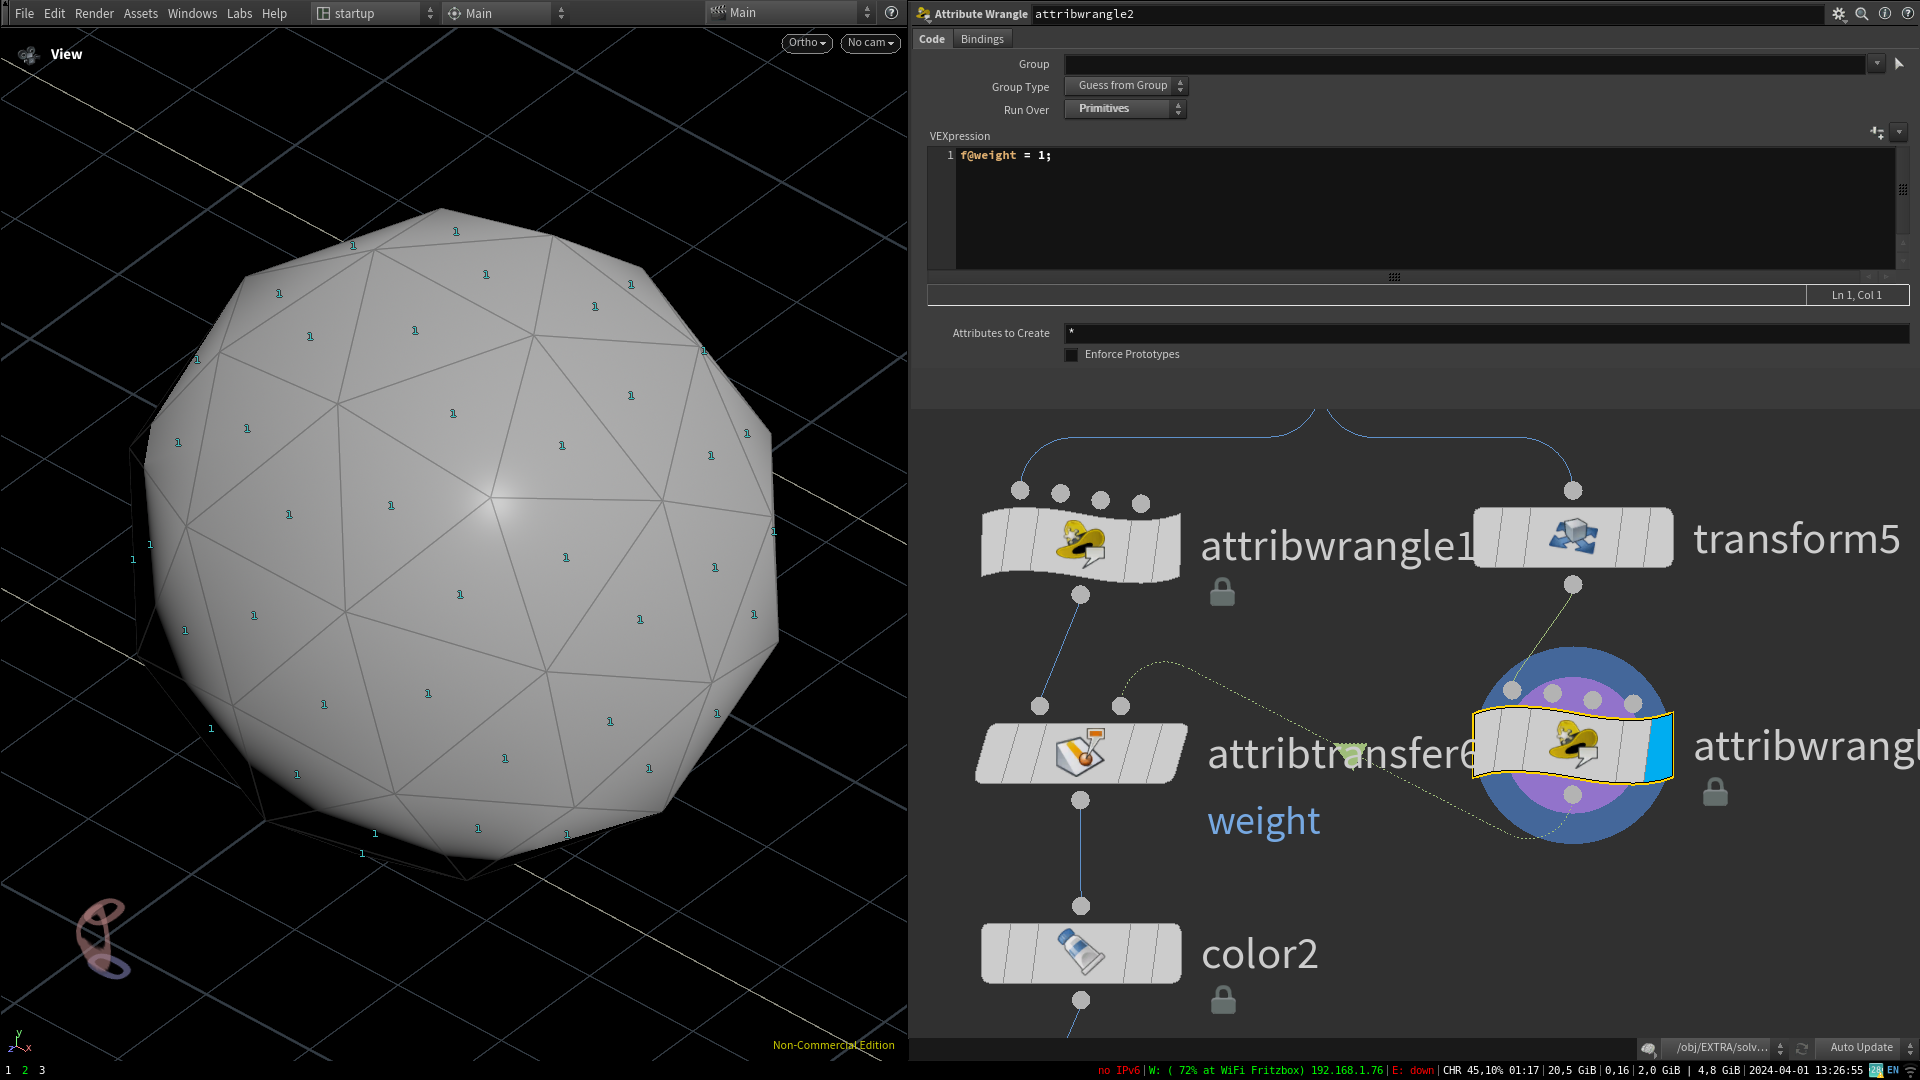
\includegraphics[width=1\textwidth]{media/houdini_fundamentals_5.png}
	\end{minipage}


	\begin{minipage}[H]{0.4\textwidth}
		\textbf{6: polyextrude SOP}\newline 
the same as the previous wrangle SOP, only with the opposite value.The reason
we interpolate between 0 and 1 is because it is easier to work with normalized
values that arbitrary values. 
	
	\end{minipage}
	\vspace{1pt}
	\begin{minipage}[H]{0.6\textwidth}
		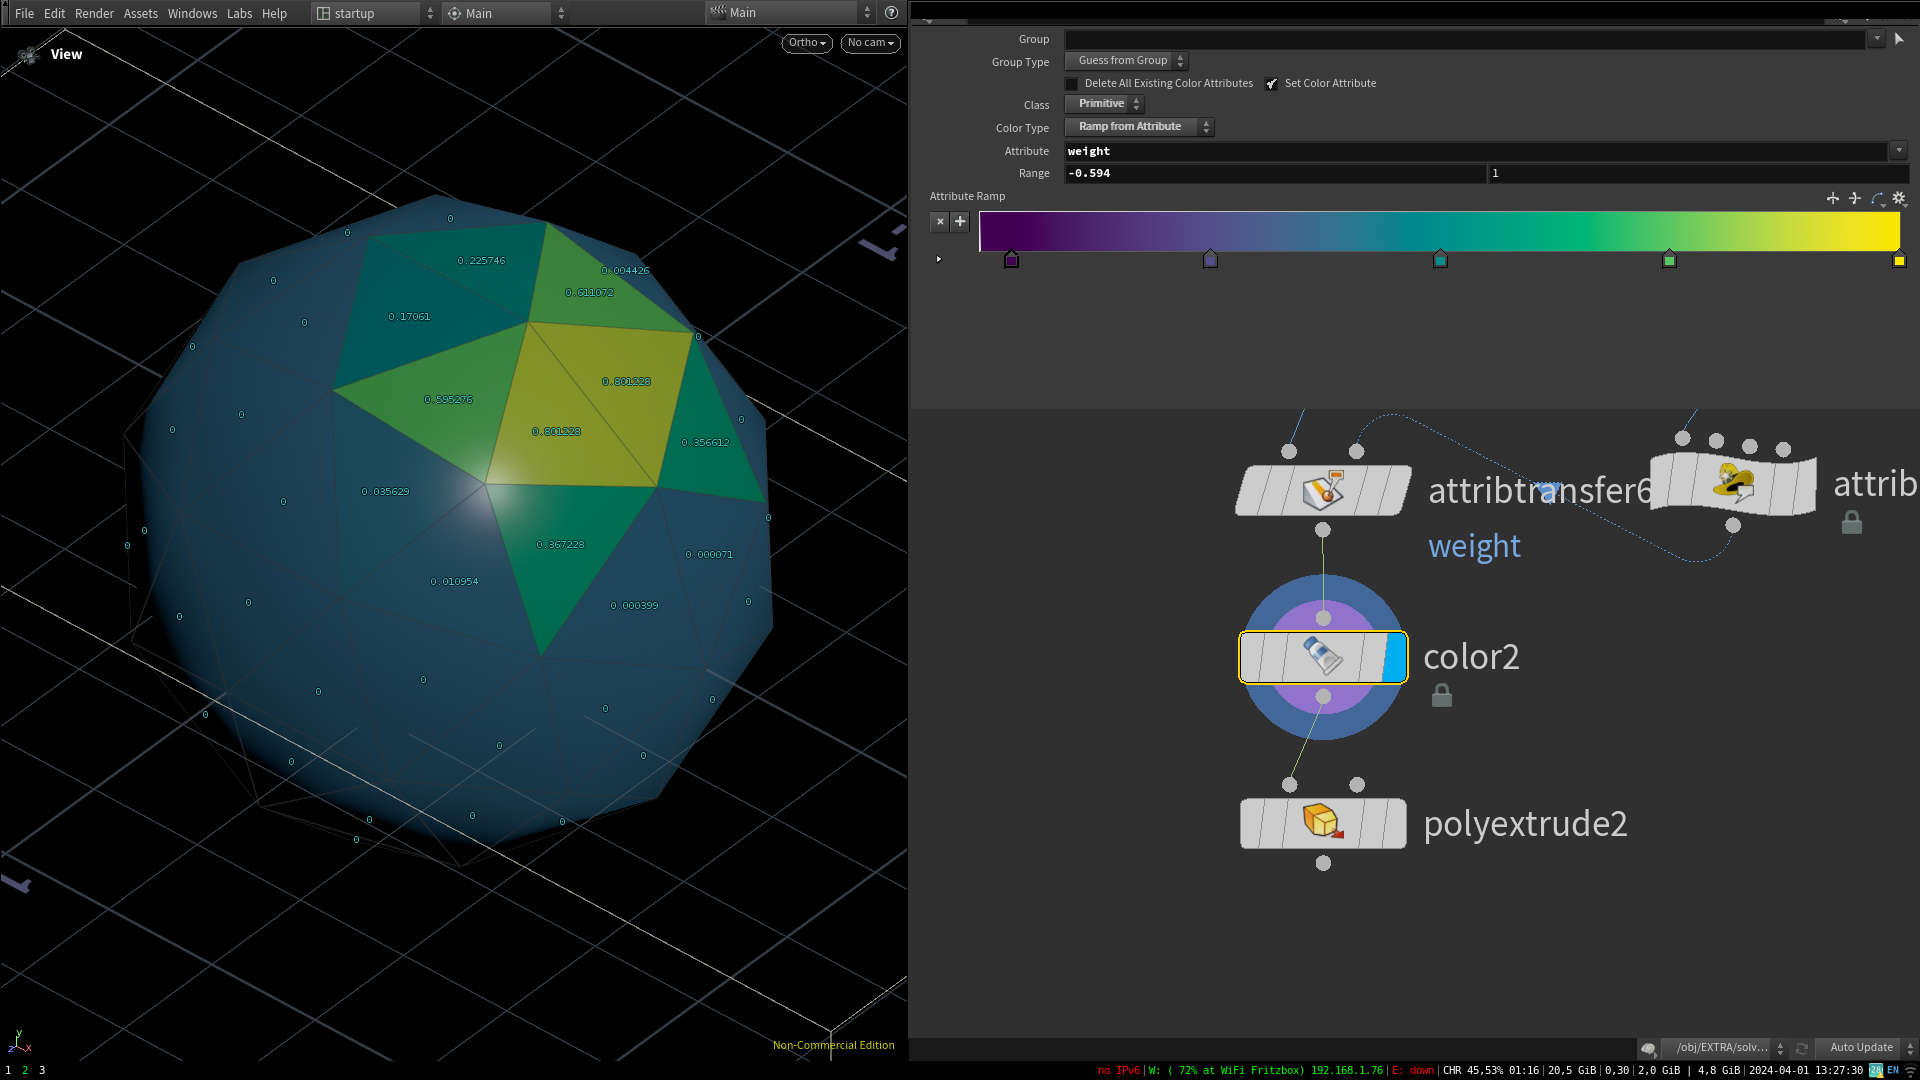
\includegraphics[width=1\textwidth]{media/houdini_fundamentals_6.png}
	\end{minipage}



	\newpage
	\section*{2.Visualizing gps and image metadata}
	
This session coveres how to overlay your google maps trajectories with images in houdini. For the assignment, the
following is expected.

	\begin{itemize}
		\item load in your own images and gps data, 
		\item generate a series of images depicting your travels.
	\end{itemize}	
	An example of such a description would be :

	\begin{figure}[H]
		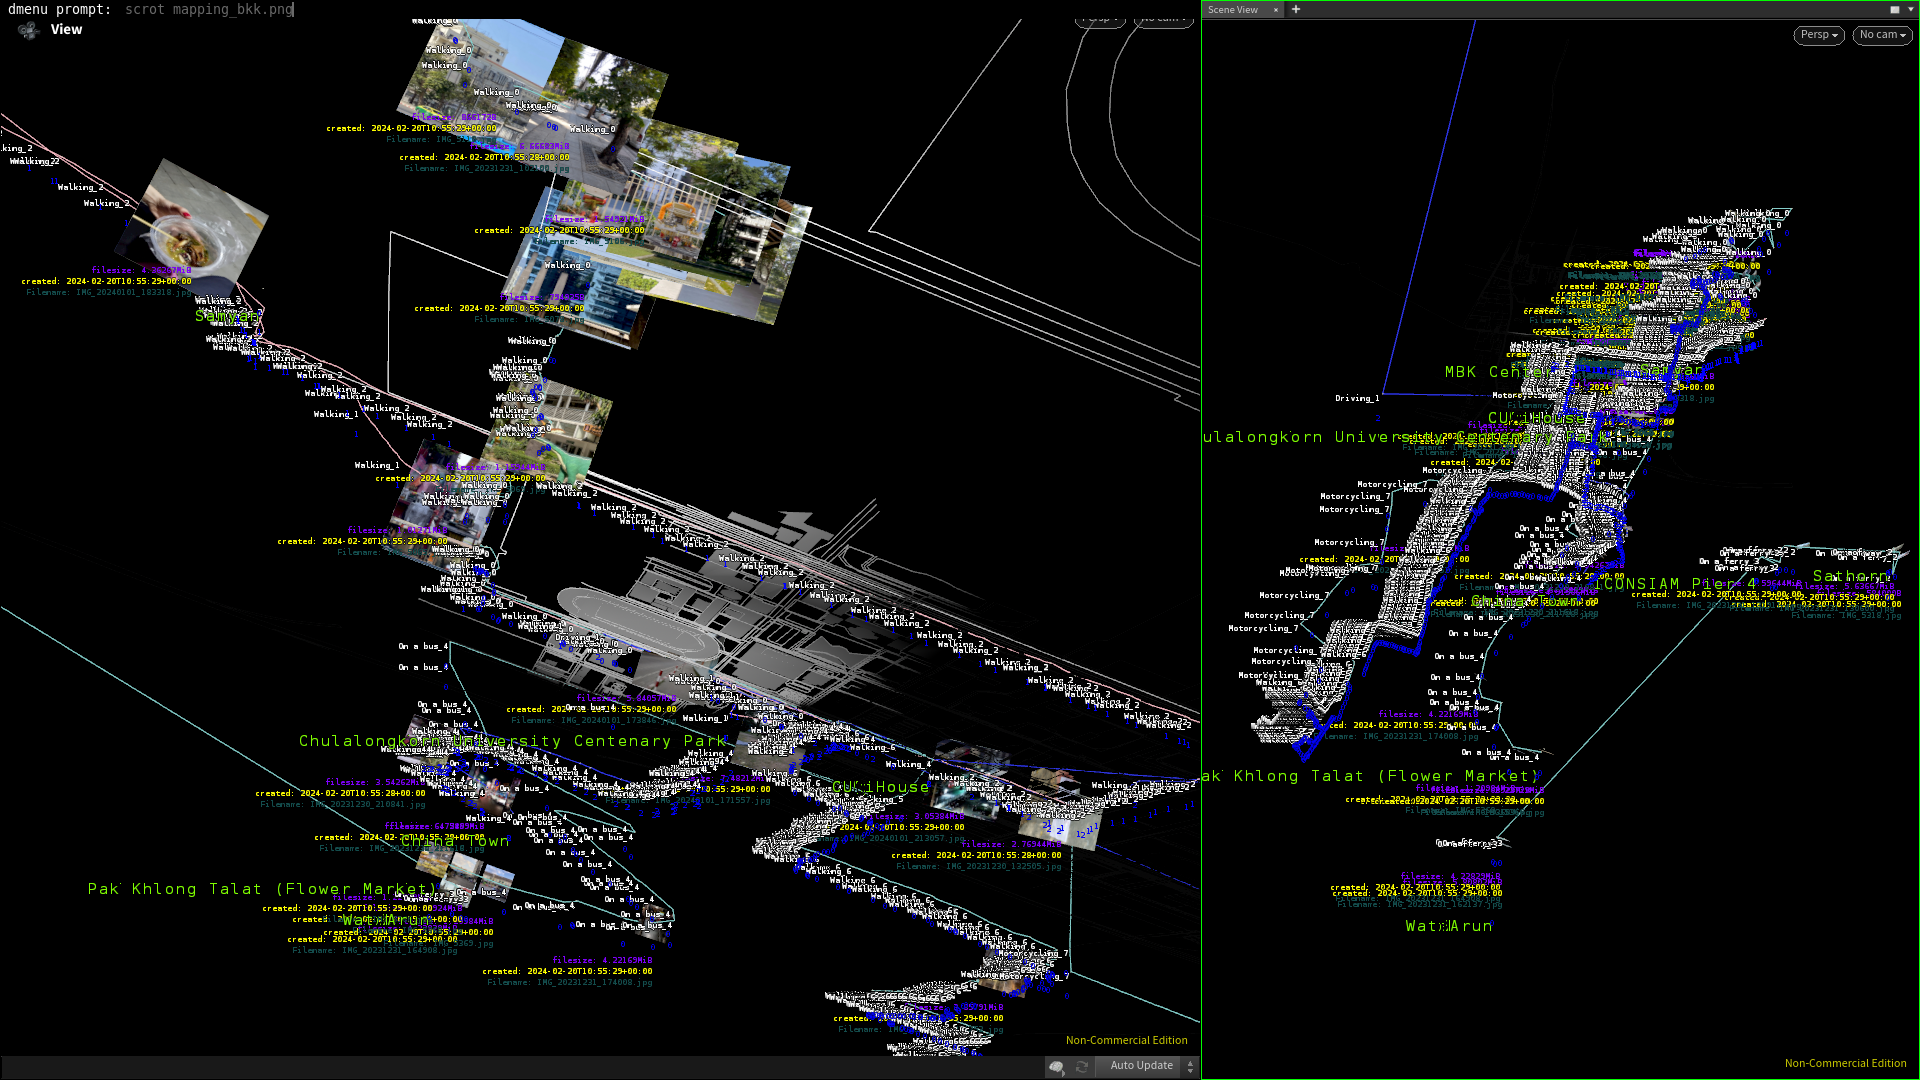
\includegraphics[width=\textwidth]{media/mapping_bkk.png}
	\end{figure}

	\begin{figure}[H]
		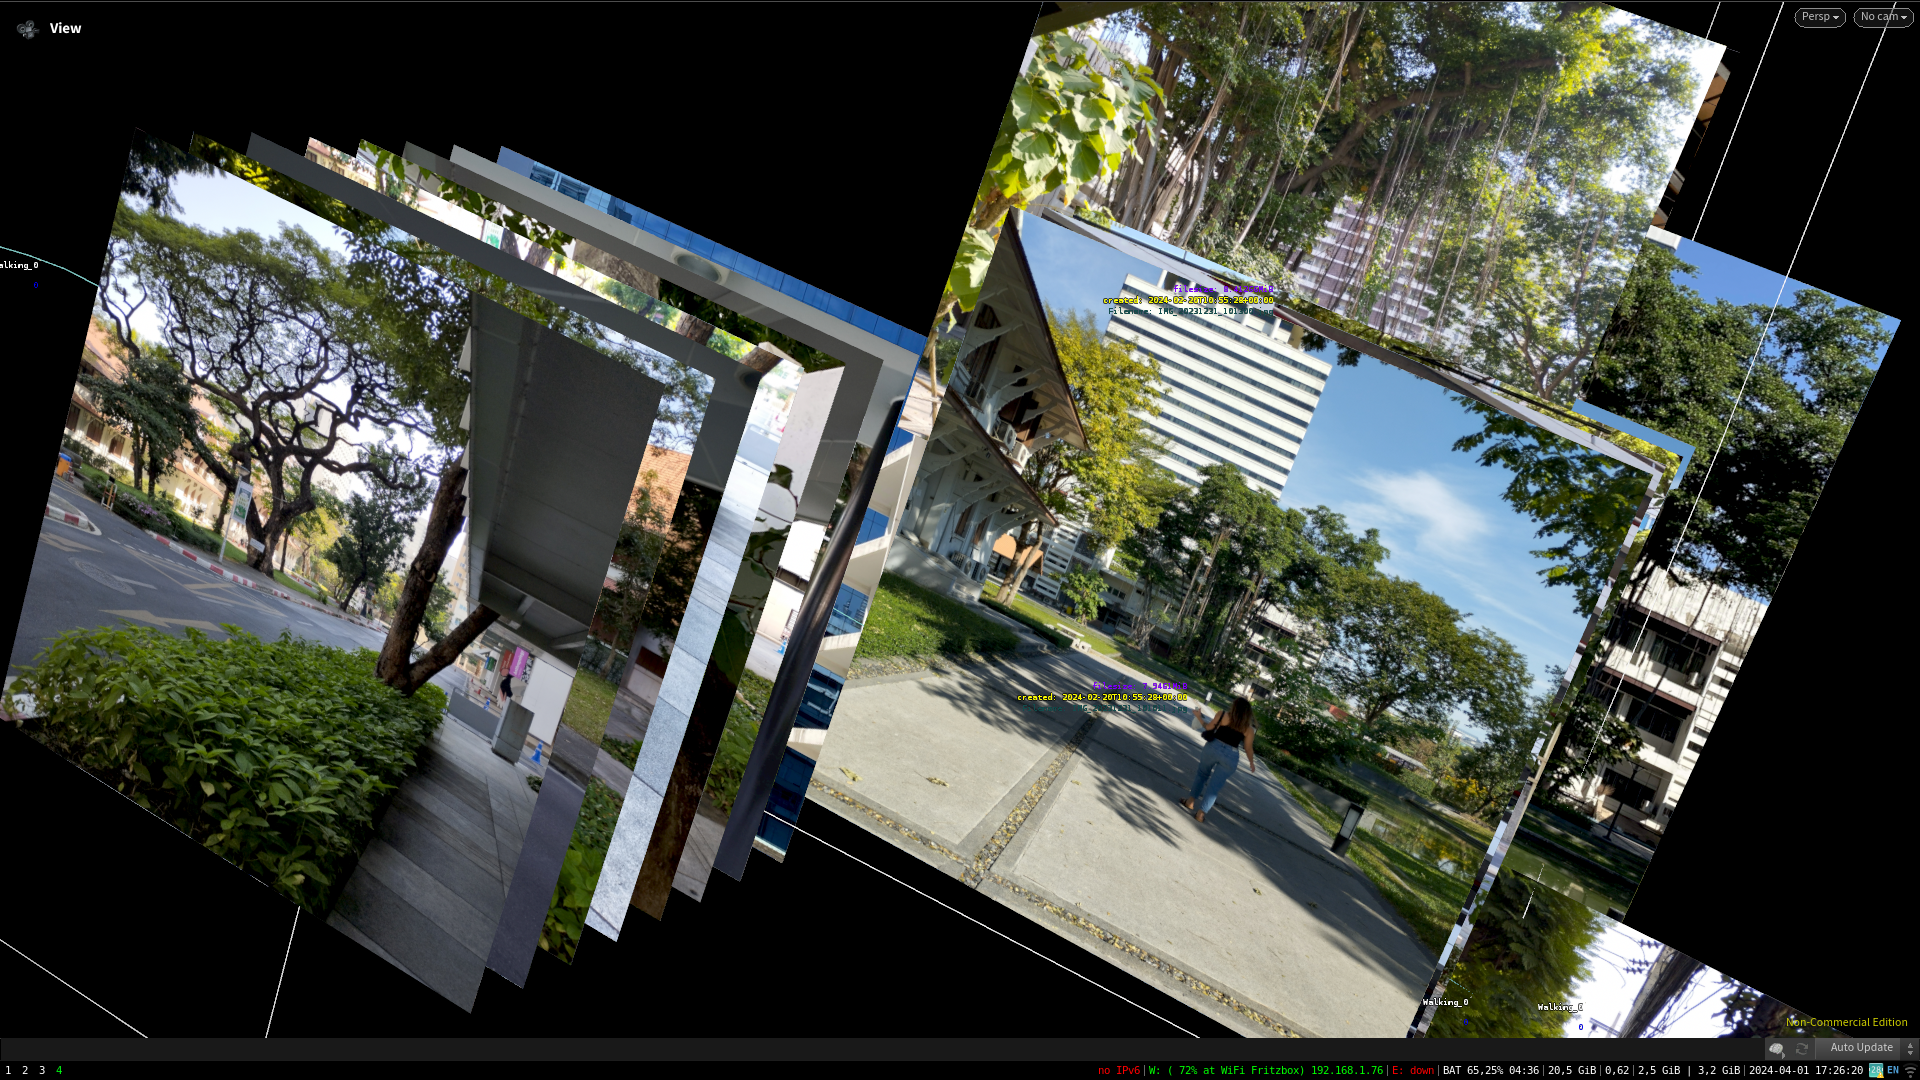
\includegraphics[width=\textwidth]{media/mapping_bkk2.png}
	\end{figure}


	\newpage
	\section*{Sora to 3d model}

In this workshop, we covered how to generate a 3d model from a video of
a subject.In this case, this was the Sora AI video published from openAI. For the assignment, the
following is expected.



	\begin{itemize}
		\item Generate one or more photogrammetry model from a video/livestream/webscraped/google images/youtube. Take footage related to your projects.
		\item reconstruct your camera path.
		\item fond a way of adding information to the subject, an additional 3d model, ) (volume specualtion, curavature, segenmbntation, adding you are sharing your entire screen sr, sharing — 	
		\item Visualize your model as a collection of images/renders.
	\end{itemize}


	\begin{figure}[h]
		  \centering
		  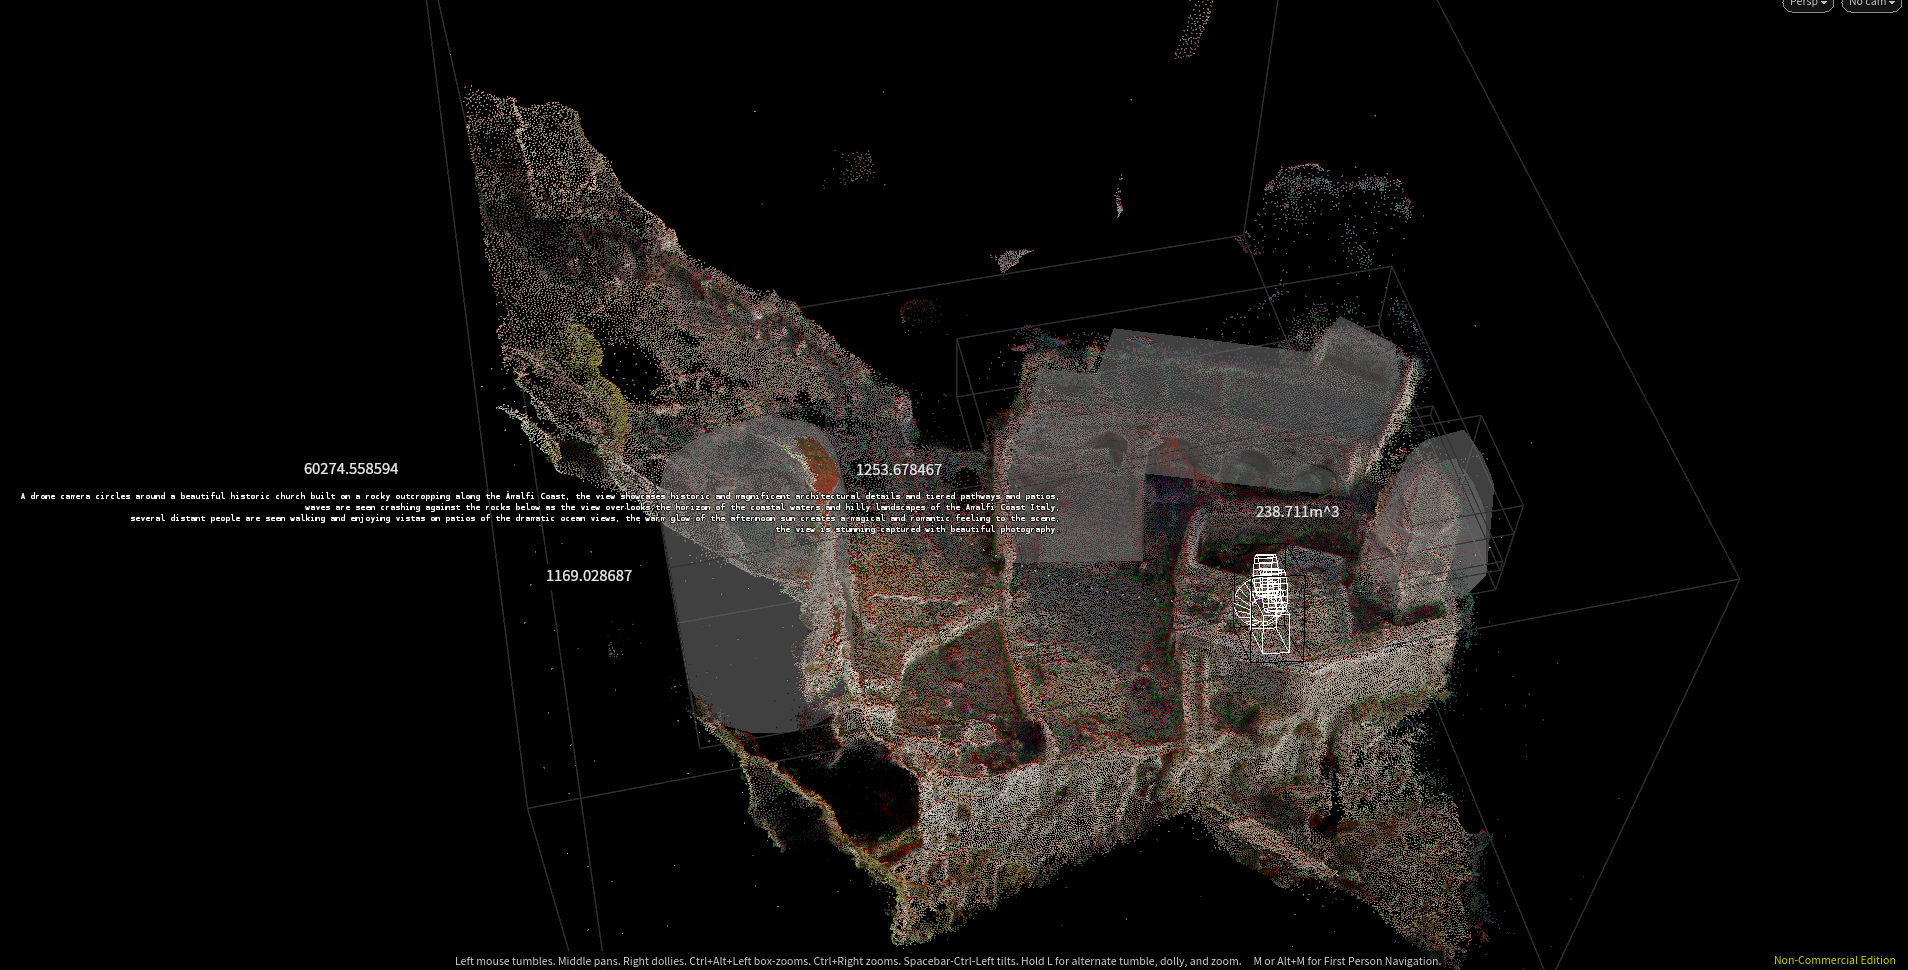
\includegraphics[width=\textwidth]{media/sora.png}
	\end{figure}



	\newpage
	\section*{visualizing json in houdini}

In this workshop, we covered how to  generate a json file that can be read and processed in
houdini. This is usefull if you are constructing a .pickle or .json file  and want to know how this can be visualized in Houdini

	\begin{itemize}
		\item based on your project/and other workshops,visualize a json file. This can take many forms. It is up to you how to shocase this in the best way.
	\end{itemize}

	\begin{figure}[h]
		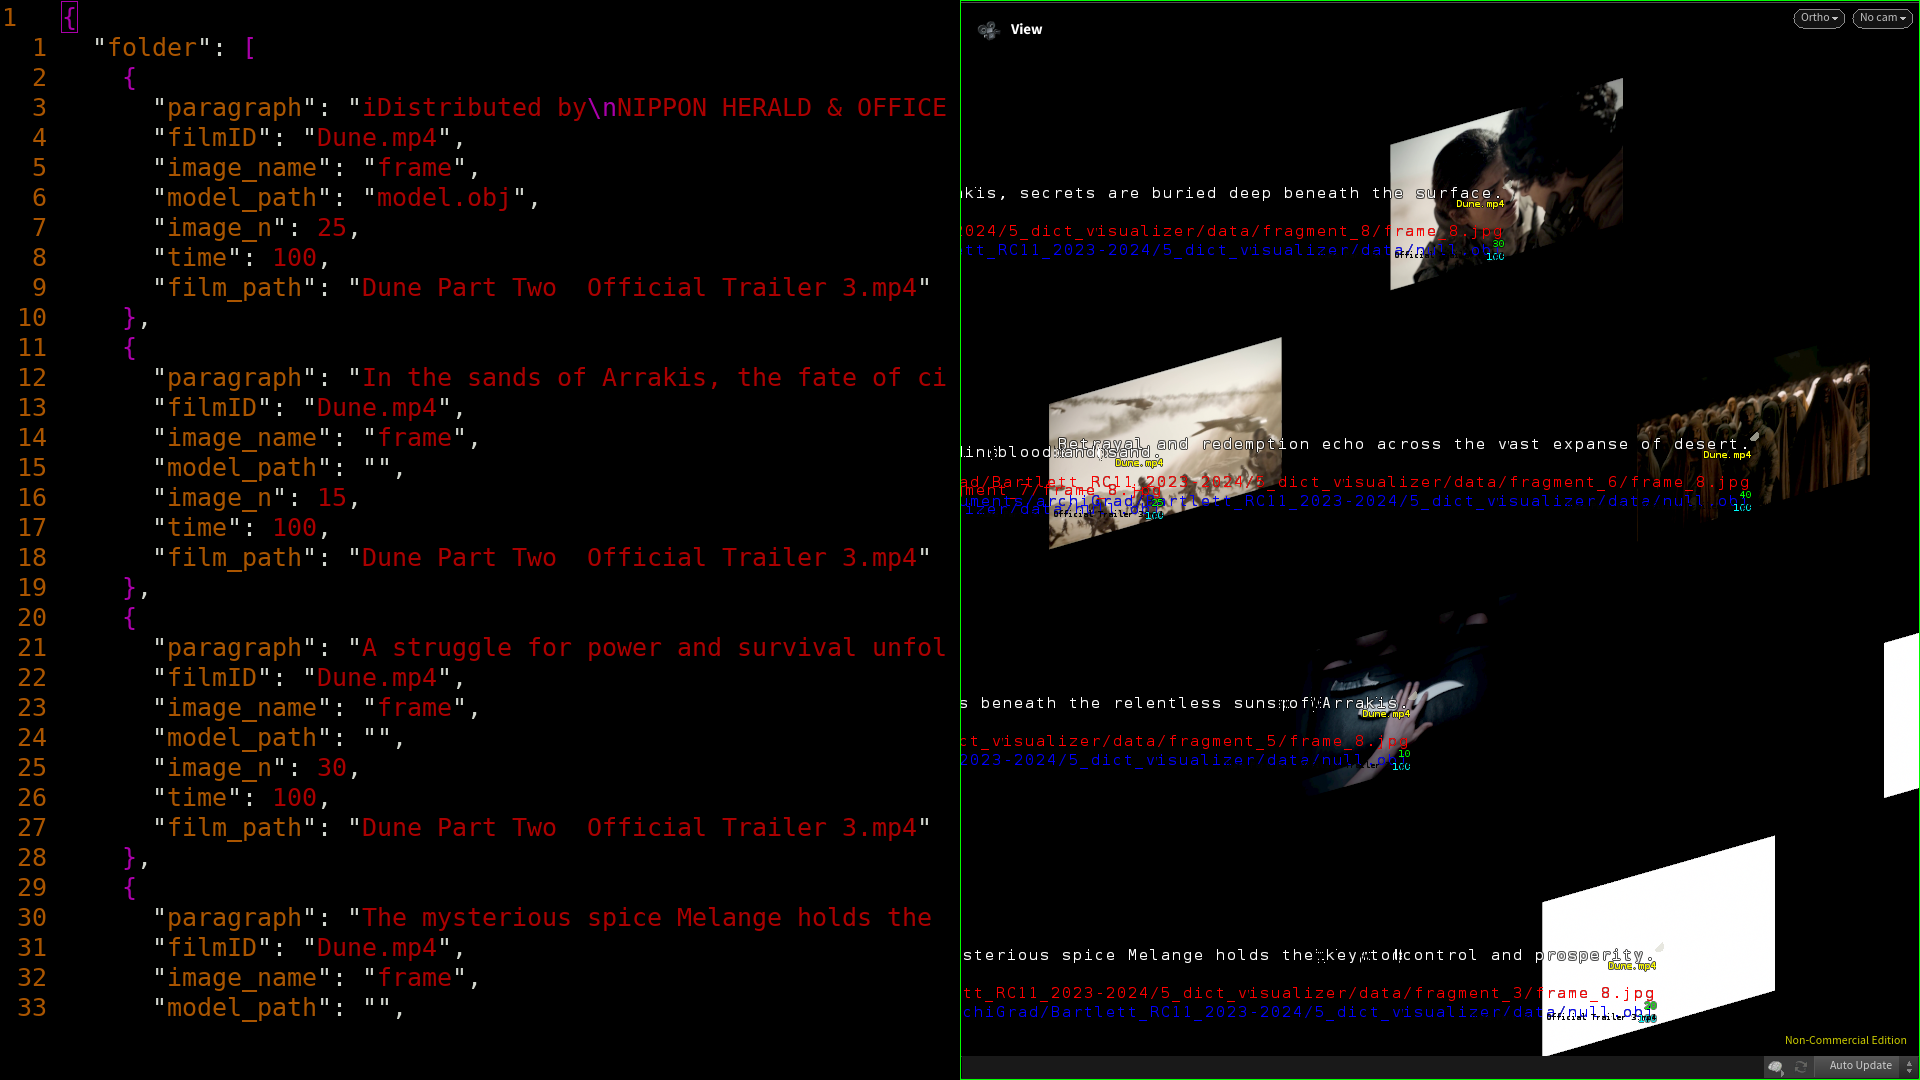
\includegraphics[width=\textwidth]{media/json_visualizer.png}
	\end{figure}

\end{document}
